\section{Data Retrieval}
Written by David Sandoz.
\subsection{Looking for data}
Initially, the project idea was to get Alps weather information from social networks using natural language processing. Hence we first looked how to mine Twitter, Facebook, Instagram or Camptocamp. We also searched for other datasources such as the \emph{Institute for Snow and Avalanche Research} (SLF), MeteoSuisse or ski resorts. After discussion and clarification with our TA, the scope and goal of our project changed in order to get closer to a \emph{Big Data} project. Hence we needed to process a big dataset and the \emph{Integrated Surface Database} from NOAA seems to be the one.

\subsection{The \emph{Integrated Surface Database}}
The \emph{National Oceanic and Atmospheric Administration} (NOAA) is the US agency responsible for the weather surveillance and forecast. They have a \emph{National Climatic Data Center} (NCDC), “responsible for preserving, monitoring, assessing, and providing public access to the Nation's treasure of climate and historical weather data and information”. One of their datasets is the \emph{Integrated Surface Database} which has data not only for the USA territories, but for the whole world (20,000 stations). We can access this dataset under the following condition, which we fulfill.
\begin{quote}
“The following data and products may have conditions placed on their international commercial use. They can be used within the U.S. or \textbf{for non-commercial international activities without restriction}. The non-U.S. data cannot be redistributed for commercial purposes. Re-distribution of these data by others must provide this same notification.”
\end{quote}
The data is accessible by FTP at \url{ftp://ftp.ncdc.noaa.gov/pub/data/noaa/} using anonymous login. There is one directory per year and within each directory one file per weather station. Within a file, one line correspond to one data record of the station at a specific time.

All stations are listed in the file \texttt{ish-history.txt} with, among other attributes, their coordinates and the country in which they are located.

Every station can have two IDs: the \emph{Air Force Datsav3 station number} (USAF) (6 figures) or the \emph{NCDC WBAN number} (WBAN) (5 figures). Most stations have only one of these two IDs (the other being set to 9s). Hence we defined the ID of a station as being the combination of the two IDs, which guarantee uniqueness.

It is important to note that despite the fact that each stations has precise coordinates, each line entry in the dataset give the coordinates again because a station might be slightly moved.

\subsection{Downloading the data}
The dataset is over 500GB large when uncompressed. As we only have 300GB on our server, we couldn't download the whole dataset. In order to have a sample dataset, we downloaded 10 years (2004-2013) of data for Switzerland, which is around 2GB large. Then we downloaded 39 years (1975-2013) of data for the USA, which is around 200GB large. We can notice that these 39 years of data for the USA are a big part of the whole dataset. We can therefore deduce that these years are richer (more frequent sampling).

\begin{figure}[htb]
	\centering
	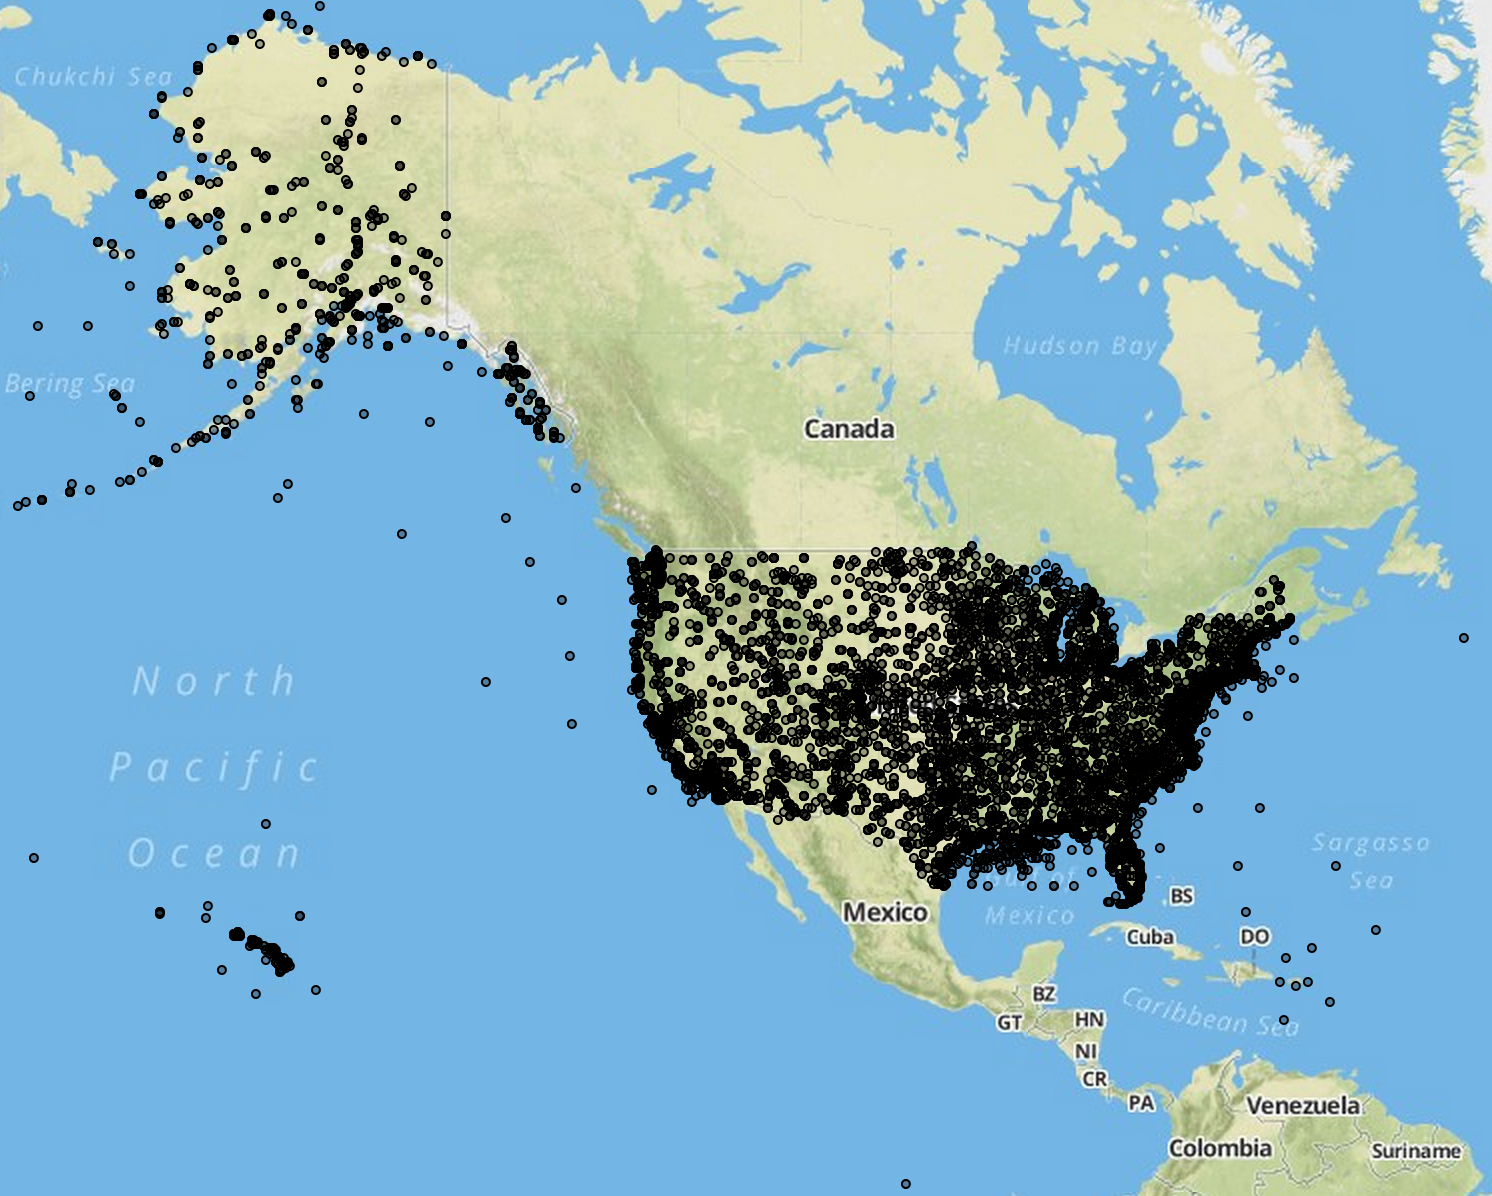
\includegraphics[width=0.9\textwidth]{figures/USStations.png}
	\caption{Stations categorized as being in the USA}
\end{figure}

To proceed the download from the NOAA FTP server to our server, we wrote a Shell script taking in argument the \texttt{filename} of a file containing a list of the stations we want and the \texttt{year} for which we want the data. As not all the stations are active all the time, there won't necessarily be a file for each station in our list. Hence, before downloading, the script computes the intersection between the stations in our list and the files available on the FTP server. This will improve the downloading as it will not ask for files which doesn't exist.